%%%
% Plantilla de Memoria
% Modificación de una plantilla de Latex de Nicolas Diaz para adaptarla 
% al castellano y a las necesidades de escribir informática y matemáticas.
%
% Editada por: Mario Román
%
% License:
% CC BY-NC-SA 3.0 (http://creativecommons.org/licenses/by-nc-sa/3.0/)
%%%

%%%%%%%%%%%%%%%%%%%%%%%%%%%%%%%%%%%%%%%%%
% Thin Sectioned Essay
% LaTeX Template
% Version 1.0 (3/8/13)
%
% This template has been downloaded from:
% http://www.LaTeXTemplates.com
%
% Original Author:
% Nicolas Diaz (nsdiaz@uc.cl) with extensive modifications by:
% Vel (vel@latextemplates.com)
%
% License:
% CC BY-NC-SA 3.0 (http://creativecommons.org/licenses/by-nc-sa/3.0/)
%
%%%%%%%%%%%%%%%%%%%%%%%%%%%%%%%%%%%%%%%%%

%----------------------------------------------------------------------------------------
%	PAQUETES Y CONFIGURACIÓN DEL DOCUMENTO
%----------------------------------------------------------------------------------------
%%% Configuración del papel.
% microtype: Tipografía.
% mathpazo: Usa la fuente Palatino.
\documentclass[a4paper, 11pt]{article}
\usepackage[protrusion=true,expansion=true]{microtype}
\usepackage{mathpazo}


% Indentación de párrafos para Palatino
\setlength{\parindent}{0pt}
  \parskip=8pt
\linespread{1.05} % Change line spacing here, Palatino benefits from a slight increase by default


%%% Castellano.
% noquoting: Permite uso de comillas no españolas.
% lcroman: Permite la enumeración con numerales romanos en minúscula.
% fontenc: Usa la fuente completa para que pueda copiarse correctamente del pdf.
\usepackage[spanish,es-noquoting,es-lcroman]{babel}
\usepackage[utf8]{inputenc}
\usepackage[T1]{fontenc}
\selectlanguage{spanish}


%%% Gráficos
\usepackage{graphicx} % Required for including pictures
\usepackage{wrapfig} % Allows in-line images
\usepackage[usenames,dvipsnames]{color} % Coloring code

%%% Matemáticas
\usepackage{amsmath}


%%% Bibliografía
\makeatletter
\renewcommand\@biblabel[1]{\textbf{#1.}} % Change the square brackets for each bibliography item from '[1]' to '1.'
\renewcommand{\@listI}{\itemsep=0pt} % Reduce the space between items in the itemize and enumerate environments and the bibliography
\usepackage{hyperref}
\hypersetup{
	colorlinks   = true,    % Colours links instead of ugly boxes
	urlcolor     = red,    % Colour for external hyperlinks
	linkcolor    = red,    % Colour of internal links
	citecolor    = blue      % Colour of citations
}

%%% CÓDIGO

\usepackage{listings}   
\usepackage{xcolor}
\lstdefinestyle{customc}{	
	backgroundcolor=\color{white},    % choose the background color; you must add \usepackage{color} or \usepackage{xcolor}; should come as last argument
	basicstyle=\footnotesize\ttfamily,% the size of the fonts that are used for the code
	breakatwhitespace=false,          % sets if automatic breaks should only happen at whitespace
	breaklines=true,                  % sets automatic line breaking
	captionpos=b,                     % sets the caption-position to bottom
    commentstyle=\itshape\color{purple!40!black},     % comment style
	deletekeywords={...},             % if you want to delete keywords from the given language
	escapeinside={\%*}{*)},           % if you want to add LaTeX within your code
	extendedchars=true,               % lets you use non-ASCII characters; for 8-bits encodings only, does not work with UTF-8
	frame=single,	                  % adds a frame around the code
	keepspaces=true,                  % keeps spaces in text, useful for keeping indentation of code (possibly needs columns=flexible)
	keywordstyle=\bfseries\color{green!40!black},       % keyword style
	language=C,                       % the language of the code
	morekeywords={*,...},             % if you want to add more keywords to the set
	numbers=left,                     % where to put the line-numbers; possible values are (none, left, right)
	numbersep=5pt,                    % how far the line-numbers are from the code
	numberstyle=\tiny\color{gray},    % the style that is used for the line-numbers
	rulecolor=\color{black},          % if not set, the frame-color may be changed on line-breaks within not-black text (e.g. comments (green here))
	showspaces=false,                 % show spaces everywhere adding particular underscores; it overrides 'showstringspaces'
	showstringspaces=false,           % underline spaces within strings only
	showtabs=false,                   % show tabs within strings adding particular underscores
	stepnumber=2,                     % the step between two line-numbers. If it's 1, each line will be numbered
    stringstyle=\color{orange},       % string literal style
	tabsize=2,	                      % sets default tabsize to 2 spaces
	title=\lstname,                   % show the filename of files included with \lstinputlisting; also try caption instead of title
	identifierstyle=\color{blue}
}

\lstdefinestyle{customasm}{
	belowcaptionskip=1\baselineskip,
	frame=L,
	xleftmargin=\parindent,
	language=[x86masm]Assembler,
	basicstyle=\footnotesize\ttfamily,
	commentstyle=\itshape\color{purple!40!black},
}

\DeclareFixedFont{\ttb}{T1}{txtt}{bx}{n}{8} % for bold
\DeclareFixedFont{\ttm}{T1}{txtt}{m}{n}{8}  % for normal


\lstdefinestyle{customPY}{
	language=Python,
	basicstyle=\ttm,
	otherkeywords={self},             % Add keywords here
	keywordstyle=\ttb\color{blue},
	emph={MyClass,__init__},          % Custom highlighting
	emphstyle=\ttb\color{red},    % Custom highlighting style
	stringstyle=\color{orange},
	frame=tb,                         % Any extra options here
	showstringspaces=false       
}

\lstset{escapechar=@,style=customc}


%% cosas 

\usepackage[margin=1in]{geometry}

\usepackage{times}


%----------------------------------------------------------------------------------------
%	TÍTULO
%----------------------------------------------------------------------------------------
% Configuraciones para el título.
% El título no debe editarse aquí.
\renewcommand{\maketitle}{
  \begin{flushright} % Right align
  
  {\LARGE\@title} % Increase the font size of the title
  
  \vspace{50pt} % Some vertical space between the title and author name
  
  {\large\@author} % Author name
  \\\@date % Date
  \vspace{40pt} % Some vertical space between the author block and abstract
  \end{flushright}
}

%% Título
\title{\textbf{Construyendo sobre Prelude}\\ % Title
					una introducción a Emacs.} % Subtitle

\author{\textsc{Francisco Navarro Morales} % Author
\\{\textit{GRG121}}} % Institution

\date{\today} % Date





%----------------------------------------------------------------------------------------
%	DOCUMENTO
%----------------------------------------------------------------------------------------

\begin{document}
	
	
	\begin{titlepage}
		\begin{center}
			\vspace*{2cm}
			
			{\Huge \textbf{Cómo resolver un Sudoku Samurai}}
			
			 ALGORITMICA 
			
			
			\vspace{0.5cm}
			
			
		    \centering 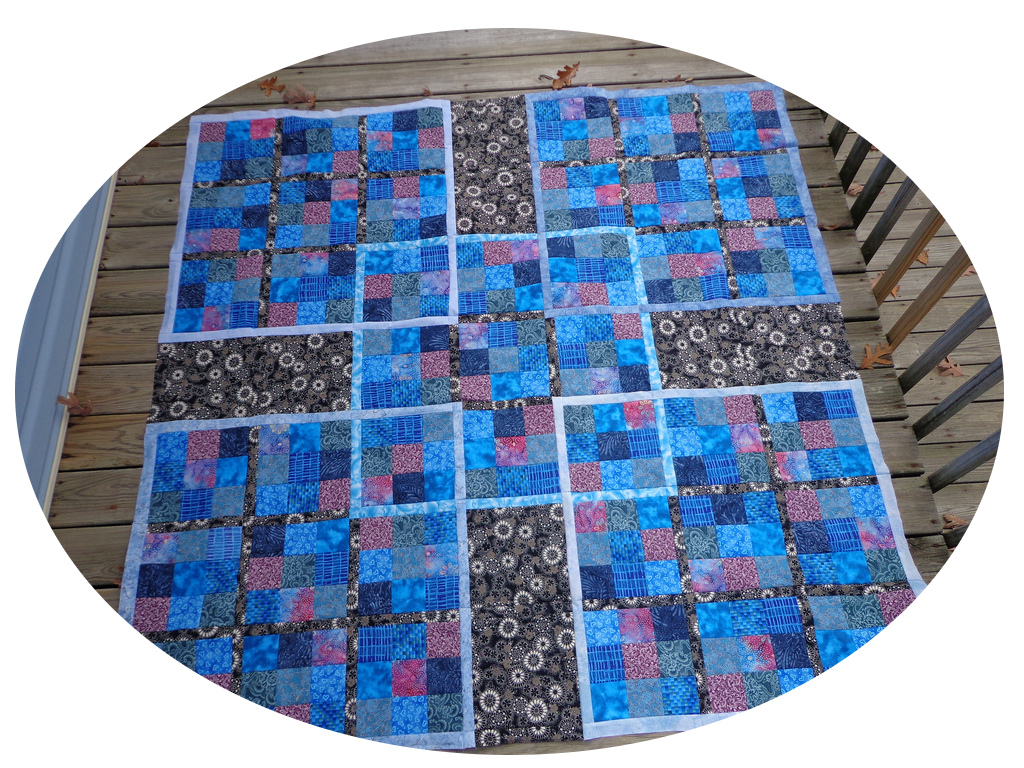
\includegraphics[width=0.9\textwidth]{cover.jpg}
		    
		    
		    {\footnotesize Photo by Scientific Quilter on Flickr}
			
			\vspace{2cm}
			
			\textbf{Francisco Navarro Morales - GRG121 }
			
			\vfill
			
			Segundo curso del Grado de Ingeniería Informática\\
			Universidad de Granada\\
			curso 2016-2017\\
			
		\end{center}
	\end{titlepage}


%\maketitle % Print the title section

%% Resumen (Descomentar para usarlo)
\renewcommand{\abstractname}{Resumen} % Uncomment to change the name of the abstract to something else
%\begin{abstract}
% Resumen aquí
%\end{abstract}

%% Palabras clave
%\hspace*{3,6mm}\textit{Keywords:} lorem , ipsum , dolor , sit amet , lectus % Keywords
%\vspace{30pt} % Some vertical space between the abstract and first section


%% Índice
%%{\parskip=2pt
%%  \tableofcontents
%%}

%%% Inicio del documento

\pagebreak



Un sudoku samurai es aquel formado por cinco sudokus convencionales colocados de forma tal que exista un sudoku 'central' cuyas esquinas están cada una conectada a uno de los sudokus restantes. Cabría por tanto pensar que su resolución es exactamente la misma que la de un sudoku normal y que, si dispusiéramos de un algoritmo para resolver sudokus, podríamos utilizarlo para completar los cinco sudokus de forma independiente. No obstante, nada nos asegura que los datos iniciales sean suficientes para que la solución a cada uno de los sudokus sea única (propiedad básica de un sudoku), sino que se nos dan datos suficientes como para poder afirmar que el sudoku samurai al completo tiene una solución única y que lo más probable sea que necesitemos utilizar 'información' de los demás sudokus para resolver cada uno de los que forman el samurai.

Para plantearse un posible algoritmo de resolución, tendríamos que adaptar el algoritmo que resolviera sudokus 'normales' para que las esquinas compartidas tuvieran en cuenta los dos sudokus de los que forman parte a la hora de comprobar la aparición de conflictos en caso de colocar determinado número en determinada casilla, es decir, tendríamos que crear un mecanismo de comunicación entre el sudoku central y los periféricos.

A la hora de resolver un sudoku samurai manualmente, el tiempo requerido aumenta enormemente, sin embargo, si realizamos un programa que lo resuelva, el tiempo requerido no debería aumentar demasiado porque, bastaría con realizar el mismo algoritmo que para un sudoku normal pero añadiendo lo que sea necesario para que las secciones compartidas tengan en cuenta las filas y columnas de los dos sudokus a los que pertenecen. Salvando ese cambio y utilizando el algoritmo no de forma independiente para cada sudoku sino a nivel global (haría falta un algoritmo que atacara el problema por secciones o adaptar uno que atacara el sudoku al completo para que actuara sobre todo el sudoku samurai), de forma tal que, en el momento en que las esquinas compartidas estuvieran resueltas o a punto de resolverse, el sudoku podría ser fácilmente completado simplemente buscando casillas en las que inequívocamente tuviera que ir un número concreto. 


\end{document}